\documentclass[10pt,letterpaper]{article}

% Reproduction de la mise en page NeurIPS (marges, police, interligne)
\usepackage[letterpaper, left=1.5in, right=1in, top=1in, bottom=1in]{geometry}
\usepackage[utf8]{inputenc}
\usepackage[T1]{fontenc}
\usepackage[french]{babel}
\usepackage{times}              % Times New Roman (proche NeurIPS)
\usepackage{hyperref}
\usepackage{url}
\usepackage{booktabs}
\usepackage{amsfonts}
\usepackage{amsmath}
\usepackage{nicefrac}
\usepackage{microtype}
\usepackage{xcolor}
\usepackage{graphicx}
\usepackage{subcaption}
\usepackage{setspace}
\usepackage{titlesec}

% Interligne NeurIPS : 11pt leading sur 10pt type
\setlength{\baselineskip}{11pt}

% Format des titres (NeurIPS : bold, flush left)
\titleformat{\section}{\normalsize\bfseries}{\thesection}{1em}{}
\titleformat{\subsection}{\normalsize\bfseries}{\thesubsection}{1em}{}
\titleformat{\subsubsection}{\normalsize\bfseries}{\thesubsubsection}{1em}{}

% Pas d'indentation, demi-ligne entre paragraphes
\setlength{\parindent}{0pt}
\setlength{\parskip}{5.5pt}

% Mise en forme de l'abstract
\renewenvironment{abstract}
  {\small\quotation\noindent\textbf{Résumé.} }
  {\endquotation}

\hypersetup{
  colorlinks=true,
  linkcolor=black,
  citecolor=black,
  urlcolor=black
}

\title{\bf Modélisation thématique des professions de foi électorales françaises (1973--1993) : LDA, NMF et BERTopic}

\author{%
  Mascret\\
  Master Humanités Numériques\\
  \texttt{mascret@etu.univ.fr}
}

\date{}

\begin{document}

\maketitle

\begin{abstract}
Nous analysons un corpus de 21\,167 professions de foi de candidats aux élections législatives françaises couvrant cinq scrutins entre 1973 et 1993. En appliquant trois méthodes de modélisation thématique -- LDA, NMF et BERTopic --, nous extrayons dix thèmes qui structurent le discours politique de cette période. Nos résultats montrent que les grandes lignes de clivage (gauche ouvrière, droite libérale, écologie émergente, extrême droite identitaire) sont restituées par les trois modèles, avec des différences notables de précision et de robustesse sémantique. L'analyse des distributions thématiques par année, par parti, par sexe et par département révèle des dynamiques politiques connues tout en offrant une lecture quantitative inédite à cette échelle. BERTopic produit les thèmes les plus cohérents, tandis que NMF offre la meilleure lisibilité des termes caractéristiques.
\end{abstract}

\section{Introduction}

Les professions de foi électorales constituent une source primaire d'une valeur exceptionnelle pour l'étude du discours politique. À la différence des programmes nationaux des partis, elles reflètent le discours de chaque candidat dans son contexte local, révélant ainsi la diversité interne des formations politiques et les adaptations rhétoriques aux enjeux territoriaux. La République française conserve l'intégralité de ces documents depuis la Troisième République ; leur numérisation progressive via la plateforme Arkindex du CEVIPOF (Sciences Po) en permet aujourd'hui le traitement automatique à grande échelle.

La période 1973--1993 est particulièrement riche sur le plan politique : elle couvre l'Union de la gauche et le Programme commun (1973--1978), la première alternance de la Ve République (1981), la cohabitation (1988) et la percée parlementaire du Front National (1993). Elle voit également l'émergence du mouvement écologiste comme acteur électoral autonome. Analyser les thèmes dominants de ces textes, leur évolution dans le temps et leur distribution selon les caractéristiques des candidats constitue donc un enjeu à la fois méthodologique et historique.

Dans ce travail, nous comparons trois familles de modèles de modélisation thématique : l'Allocation de Dirichlet Latente (LDA), la Factorisation de Matrice Non-négative (NMF) et BERTopic. Ces trois approches reposent sur des représentations textuelles fondamentalement différentes -- sac-de-mots probabiliste, décomposition TF-IDF, plongements de phrases neuronaux -- et leurs résultats sont confrontés de manière systématique. Nous explorons ensuite les distributions thématiques selon l'année du scrutin, le parti, le sexe, la tranche d'âge et le département du candidat.

\section{État de l'art}

\subsection{Modélisation thématique}

La modélisation thématique (\textit{topic modeling}) vise à découvrir de manière non supervisée des structures latentes dans un corpus textuel. Blei, Ng et Jordan [1] introduisent LDA, un modèle graphique probabiliste bayésien dans lequel chaque document est une mixture de thèmes, eux-mêmes définis comme des distributions sur le vocabulaire. LDA reste un point de référence incontournable en raison de sa fondation théorique solide et de son implémentation efficace via l'inférence variationnelle ou l'échantillonnage de Gibbs.

La NMF, proposée initialement par Lee et Seung [2] pour la représentation d'images, a été rapidement adaptée à la modélisation thématique [10]. En décomposant la matrice TF-IDF en deux matrices non-négatives, elle produit des thèmes souvent plus parcimonieux et interprétables que LDA, car la contrainte de non-négativité force des représentations purement additives. Arora, Ge et Moitra [11] ont montré que, sous des hypothèses d'ancrabilité (\textit{anchor words}), NMF est identifiable de façon exacte.

BERTopic [3] représente une rupture paradigmatique : au lieu de modéliser la distribution des mots, il encode chaque document dans un espace sémantique dense grâce à un transformeur pré-entraîné (Sentence-BERT [4]), réduit la dimensionnalité avec UMAP [5] et regroupe les documents avec HDBSCAN [6]. Les termes caractéristiques de chaque thème sont ensuite extraits par c-TF-IDF. Cette approche a montré des gains importants de cohérence sémantique par rapport aux approches sac-de-mots [15].

La qualité des modèles thématiques se mesure classiquement par la perplexité (LDA) et par des métriques de cohérence [7] telles que $C_V$, $C_{UCI}$, $C_{NPMI}$ et $U_{Mass}$. Ces métriques quantifient à quel point les termes d'un même thème apparaissent fréquemment ensemble dans un corpus de référence.

\subsection{Applications en sciences politiques}

La fouille de textes politiques bénéficie d'une longue tradition. Laver et Garry [9] ont montré que la comparaison des fréquences lexicales entre documents permet d'estimer les positions idéologiques des partis. Grimmer et Stewart [8] dressent un panorama des méthodes quantitatives appliquées aux textes politiques et insistent sur la complémentarité entre induction automatique de thèmes et validation qualitative par des spécialistes.

Plus récemment, l'application de transformeurs multilingues aux textes politiques a ouvert des perspectives nouvelles pour l'analyse comparée [16]. Appliqué aux corpus français, Devlin et al. [16] ont montré l'intérêt des représentations contextuelles pour les tâches de classification et d'extraction d'information. Le corpus de professions de foi du CEVIPOF reste cependant peu exploité par les méthodes d'apprentissage automatique, faisant de ce travail l'une des premières analyses thématiques automatisées à grande échelle sur ce matériau.

\section{Données et corpus}

\subsection{Description du corpus}

Le corpus provient des archives électorales numérisées par le CEVIPOF et accessibles via la plateforme Arkindex. Il comprend les professions de foi des candidats aux élections législatives pour cinq années : 1973, 1978, 1981, 1988 et 1993. Après filtrage et appariement entre les fichiers texte (issus de la reconnaissance optique de caractères) et les métadonnées du fichier \texttt{archelect\_search.csv} (33\,032 entrées au total), nous obtenons 21\,167 documents exploitables.

\begin{figure}[h]
  \centering
  \begin{subfigure}[b]{0.47\linewidth}
    \centering
    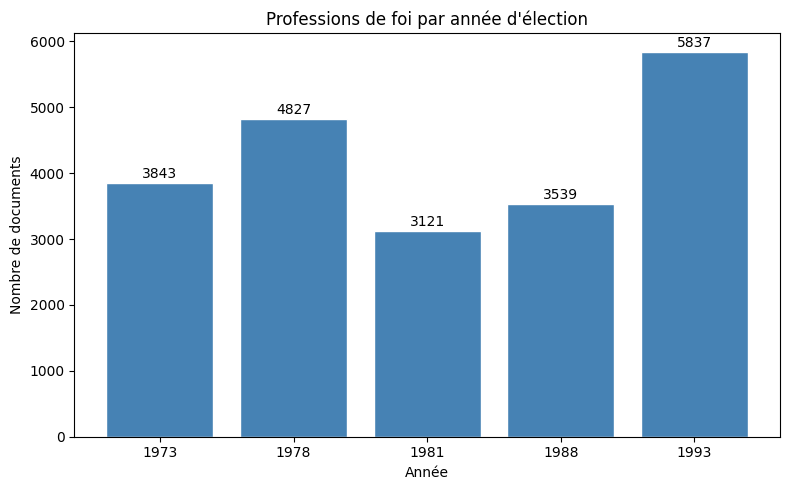
\includegraphics[width=\linewidth]{figure/figure_1.png}
    \caption{Nombre de documents par année électorale. La hausse en 1993 reflète l'augmentation des candidatures, notamment du FN.}
    \label{fig:docs_annee}
  \end{subfigure}
  \hfill
  \begin{subfigure}[b]{0.47\linewidth}
    \centering
    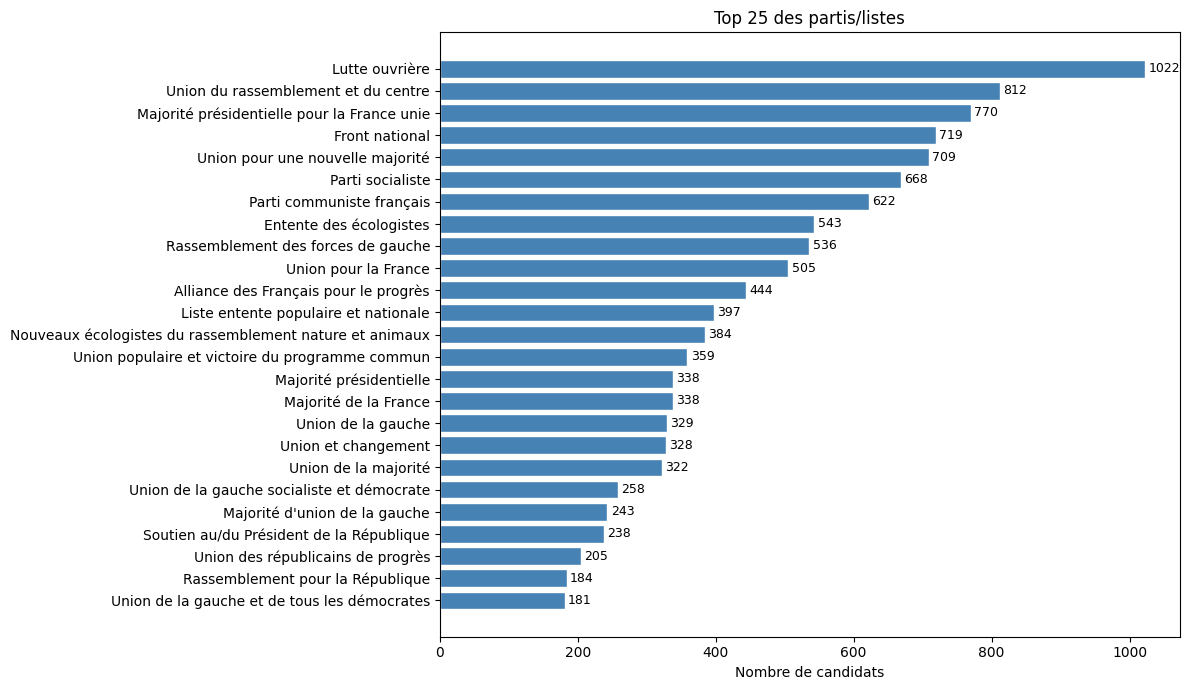
\includegraphics[width=\linewidth]{figure/figure_2.png}
    \caption{Répartition des 25 premiers partis. PS, PCF, RPR et UDF dominent, représentant plus de 60\% du corpus.}
    \label{fig:partis}
  \end{subfigure}
  \caption{Composition du corpus : 21\,167 professions de foi issues de cinq scrutins législatifs (1973--1993).}
\end{figure}

Comme le montre la Figure~\ref{fig:docs_annee}, le nombre de documents croît sensiblement sur la période, passant d'environ 2\,800 à plus de 5\,000 par scrutin, en lien avec la multiplication des candidatures, notamment du Front National à partir de 1988. Les quatre formations principales -- PS, PCF, RPR et UDF -- représentent ensemble plus de 60\% du corpus (Figure~\ref{fig:partis}).

Les métadonnées associées à chaque document incluent : le parti (reconstitué à partir des champs \textit{liste} et \textit{soutien}), le sexe, la tranche d'âge, la profession, le statut de sortant, et le département (via la cote archivistique du document).

\begin{figure}[h]
  \centering
  \begin{subfigure}[b]{0.30\linewidth}
    \centering
    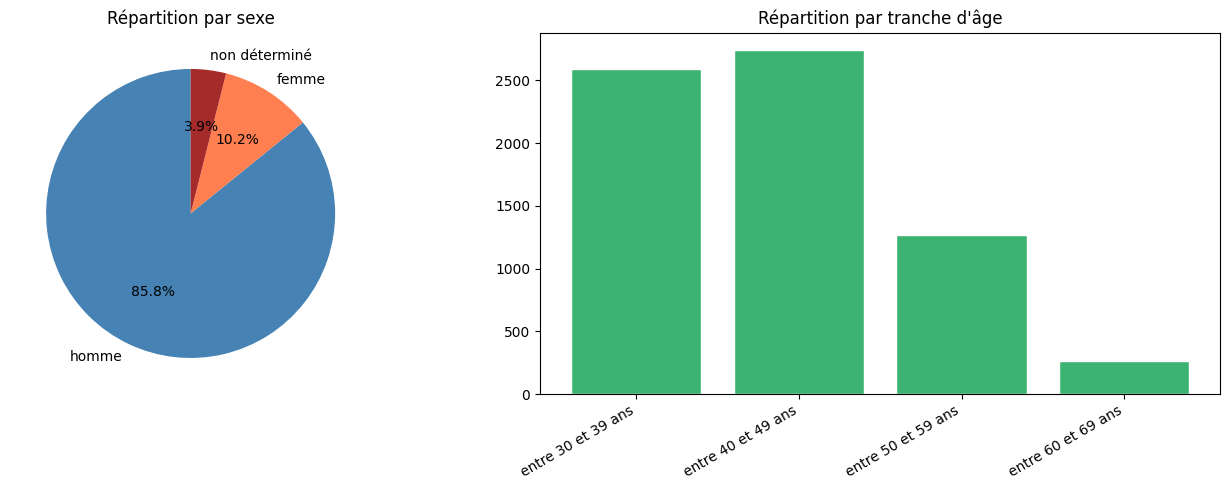
\includegraphics[width=\linewidth]{figure/figure_3.png}
    \caption{Distribution par sexe.}
    \label{fig:sexe}
  \end{subfigure}
  \hfill
  \begin{subfigure}[b]{0.30\linewidth}
    \centering
    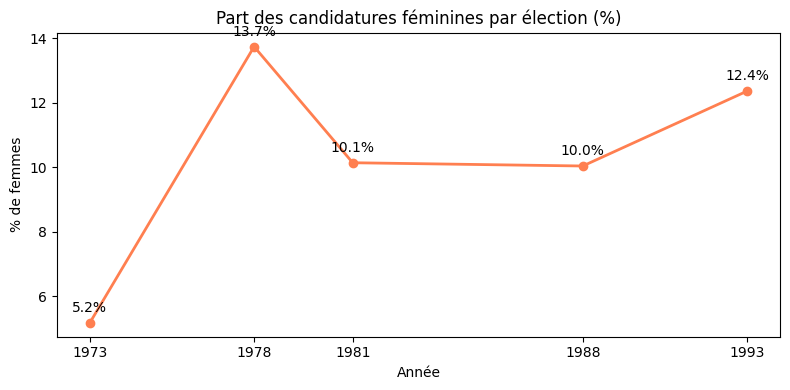
\includegraphics[width=\linewidth]{figure/figure_4.png}
    \caption{Distribution par tranche d'âge.}
    \label{fig:age}
  \end{subfigure}
  \hfill
  \begin{subfigure}[b]{0.33\linewidth}
    \centering
    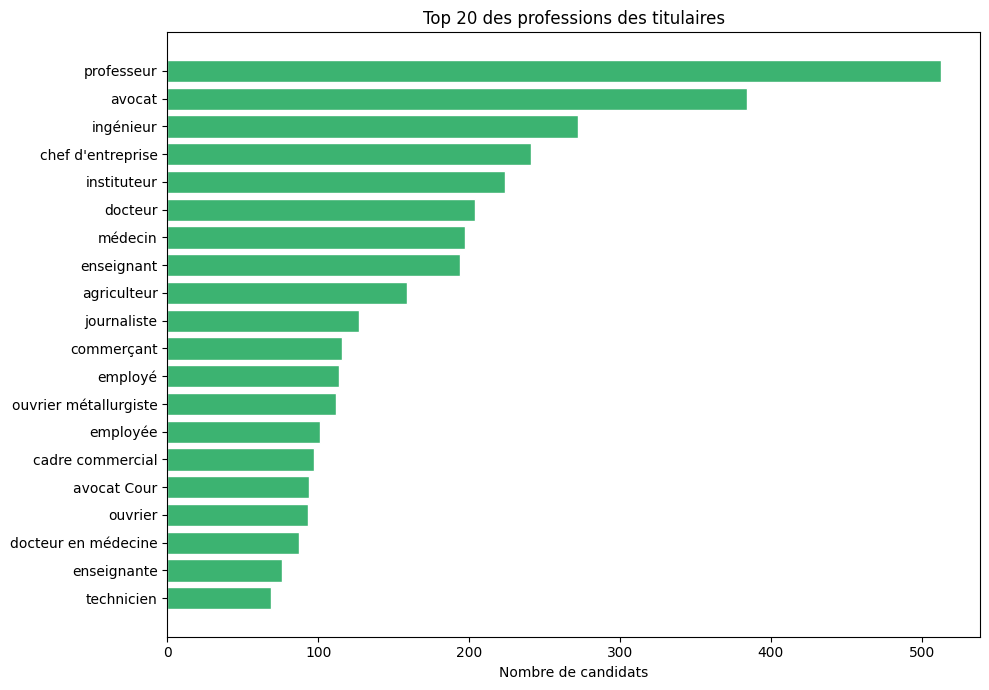
\includegraphics[width=\linewidth]{figure/figure_5.png}
    \caption{Évolution des candidatures féminines (1973--1993).}
    \label{fig:feminisation}
  \end{subfigure}
  \caption{Caractéristiques socio-démographiques du corpus. Les femmes ne représentent qu'environ 10\% des candidats, mais leur part augmente régulièrement sur la période.}
\end{figure}

La Figure~\ref{fig:sexe} illustre la forte sous-représentation féminine, cohérente avec la réalité de la vie politique française de l'époque. La Figure~\ref{fig:feminisation} montre néanmoins une tendance à la féminisation progressive, avec une accélération notable après 1988.

\subsection{Prétraitement}

Les textes bruts issus de l'OCR comportent des artefacts typiques : erreurs de segmentation, mots coupés, résidus de mise en page. Le prétraitement comprend les étapes suivantes :

(1) \textbf{Lemmatisation} via le modèle \texttt{fr\_core\_news\_sm} de spaCy [13] : les formes fléchies sont ramenées à leur lemme, réduisant la dispersion lexicale liée à la morphologie flexionnelle du français.

(2) \textbf{Normalisation des accents} : normalisation NFD suivie de filtrage des caractères combinants, harmonisant les textes selon leur qualité d'OCR.

(3) \textbf{Filtrage des mots vides} : application d'une liste de 160 mots vides français augmentée de termes spécifiques au domaine (noms de partis, formules rhétoriques récurrentes, noms de politiciens, mots allemands pour les documents alsaciens).

(4) \textbf{Filtrage par fréquence} : les termes apparaissant dans moins de 5 documents (LDA) ou 50 documents (NMF) sont écartés, de même que les termes présents dans plus de 95\% des documents.

\section{Méthodes}

\subsection{LDA -- Allocation de Dirichlet Latente}

La LDA est configurée avec $K=10$ thèmes. Le texte est représenté par un vecteur de comptages (CountVectorizer, 1\,000 features au maximum, \texttt{min\_df}=5, \texttt{max\_df}=0.95) et l'algorithme utilise un apprentissage en ligne (\textit{online} EM) sur 10 itérations. Les hyperparamètres $\alpha$ (prior sur les distributions document-thème) et $\beta$ (prior sur les distributions thème-mot) sont estimés par maximum de vraisemblance. Le choix de $K=10$ résulte d'une comparaison de la cohérence $C_V$ pour $K \in \{5, 10, 15\}$.

\subsection{NMF -- Factorisation de Matrice Non-négative}

La NMF décompose la matrice TF-IDF (TfidfVectorizer, 2\,000 features, \texttt{min\_df}=50, \texttt{max\_df}=0.95) en deux matrices $W \in \mathbb{R}^{n \times K}_+$ (documents $\times$ thèmes) et $H \in \mathbb{R}^{K \times m}_+$ (thèmes $\times$ mots), telles que $X \approx WH$. La matrice $W$ est ensuite normalisée ligne à ligne pour obtenir des distributions thématiques comparables. Le thème dominant de chaque document est celui correspondant à la valeur maximale de sa ligne dans $W$. L'optimisation utilise la descente de gradient coordonnée avec $K=10$.

\subsection{BERTopic}

BERTopic combine trois composantes distinctes :

\textbf{Encodage sémantique.} Chaque document est encodé par le modèle \texttt{paraphrase-multilingual-} \texttt{MiniLM-L12-v2} (384 dimensions), pré-entraîné par apprentissage contrastif sur plus de 50 langues. Ce modèle capture la sémantique de phrases entières, contrairement aux approches sac-de-mots.

\textbf{Réduction de dimensionnalité.} UMAP réduit les représentations 384-dimensionnelles à 15 dimensions avec 5 voisins proches, préservant à la fois la structure locale et la structure globale du manifold.

\textbf{Clustering et extraction de thèmes.} HDBSCAN (\texttt{min\_cluster\_size}=10) regroupe les documents en clusters denses. Les thèmes sont représentés par leurs termes via c-TF-IDF, une variante qui pondère les termes par leur spécificité au cluster plutôt qu'au corpus global. Le modèle produit initialement 262 micro-thèmes, réduits à 10 thèmes principaux par fusion hiérarchique agglomérative.

\section{Résultats}

\subsection{Thèmes extraits et interprétation}

Le Tableau~\ref{tab:topics} présente les dix thèmes identifiés par chacun des trois modèles, avec une étiquette interprétative dérivée des termes les plus caractéristiques. Les termes principaux illustratifs sont donnés pour NMF.

\begin{table}[h]
  \caption{Thèmes extraits par LDA, NMF et BERTopic sur le corpus des professions de foi 1973--1993. Les étiquettes sont attribuées manuellement.}
  \label{tab:topics}
  \centering
  \small
  \begin{tabular}{clll}
    \toprule
    \# & LDA & NMF (termes principaux) & BERTopic \\
    \midrule
    0 & Travail et patronat & Gauche autogestionnaire (\textit{ouvrier, socialisme, PSU}) & Gauche et travail national \\
    1 & Gauche révolutionnaire & Extrême droite FN (\textit{front, antisocialiste}) & Écologie \\
    2 & Programme commun & Lutte Ouvrière (\textit{Laguiller, femme, bombe atomique}) & Droits des travailleurs \\
    3 & Immigration FN & Écologie animale (\textit{animaux, corrida, nature}) & Lutte ouvrière et syndicats \\
    4 & Écologie et société & Immigration FN (\textit{immigré, insécurité, retablir}) & Travail et socialisme \\
    5 & Travail et énergie & Écologie politique (\textit{verts, planète, génération}) & Majorité républicaine \\
    6 & Alsace (bilingue) & Majorité présidentielle (\textit{maire, suffrage, République}) & Questions européennes \\
    7 & Majorité présidentielle & Gauche anticapitaliste (\textit{patronat, bourgeoisie, sacrifice}) & Criminalité et lois \\
    8 & Centre-droite libéral & Centre-droit (\textit{emploi, liberté, europe, développement}) & Alsace (UND/WIF) \\
    9 & Gauche diverse & Programme commun (\textit{commun, changement, victoire}) & Gauche radicale \\
    \bottomrule
  \end{tabular}
\end{table}

Les trois modèles convergent sur les grandes familles thématiques : le clivage travail/patronat, l'écologie, l'immigration portée par le FN, et le discours de la majorité présidentielle. BERTopic isole plus nettement le thème alsacien (documents comportant de l'allemand dialectal), invisible dans LDA qui le mélange avec d'autres documents. NMF distingue plus finement les nuances internes à la gauche (PS, PCF, PSU, Lutte Ouvrière), grâce à la sparsité de la décomposition.

\begin{figure}[h]
  \centering
  \begin{subfigure}[b]{0.48\linewidth}
    \centering
    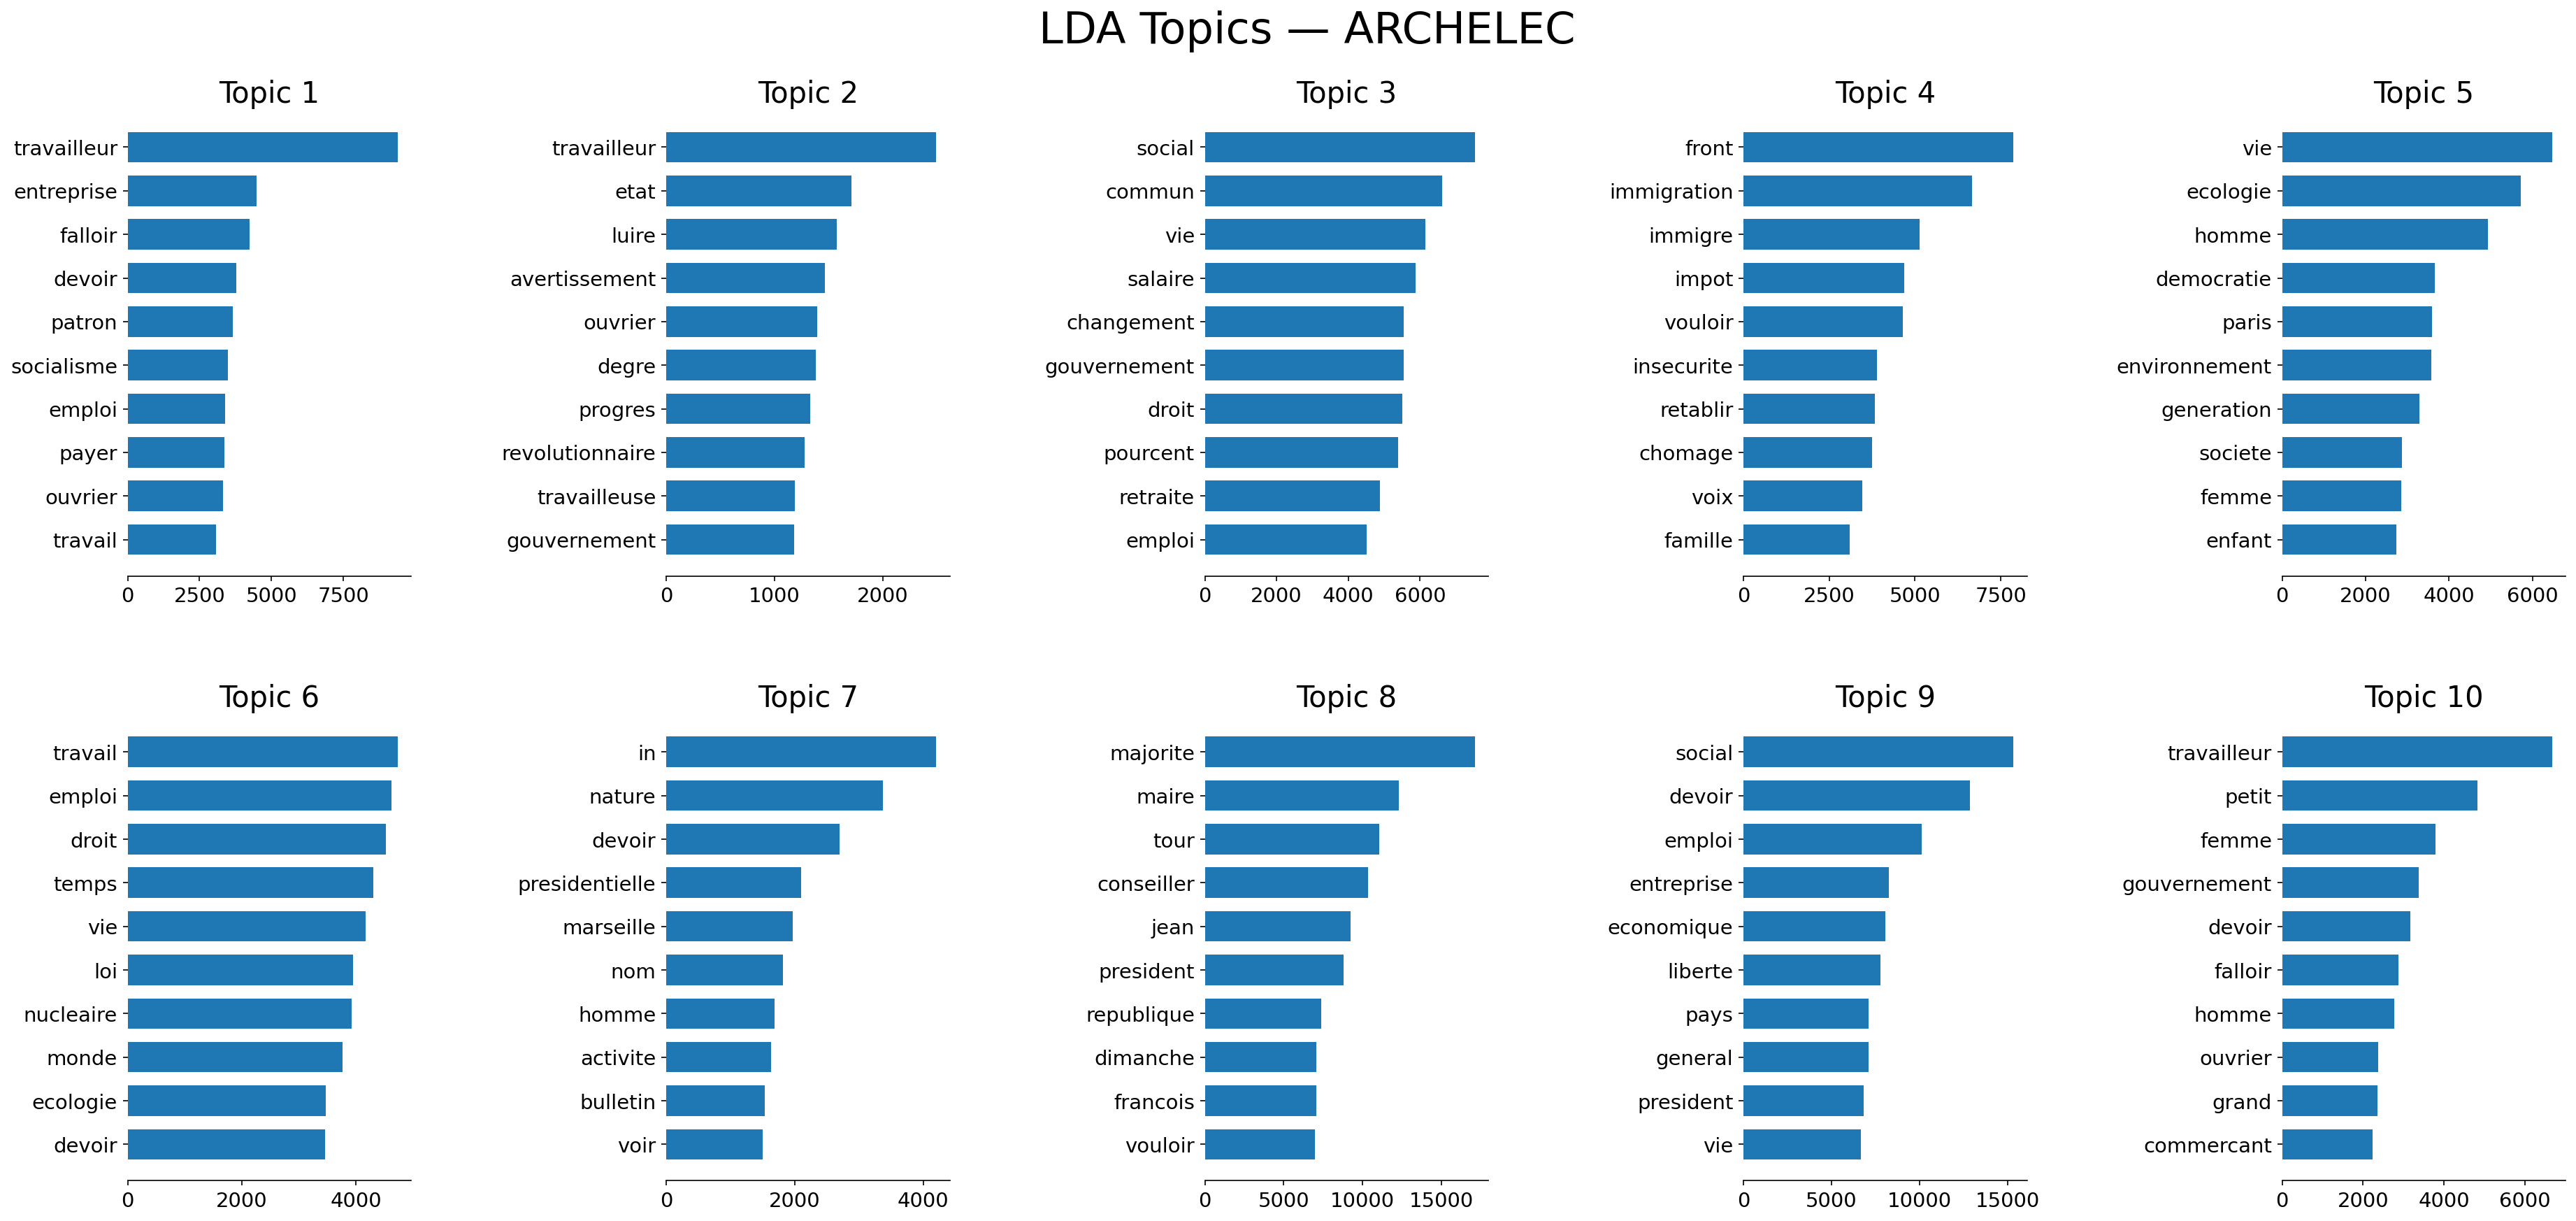
\includegraphics[width=\linewidth]{figure/figure_6.png}
    \caption{Top mots par thème (LDA). Les thèmes se chevauchent fréquemment autour du lexique du travail (\textit{travailleur} apparaît dans 5 thèmes).}
    \label{fig:lda_words}
  \end{subfigure}
  \hfill
  \begin{subfigure}[b]{0.48\linewidth}
    \centering
    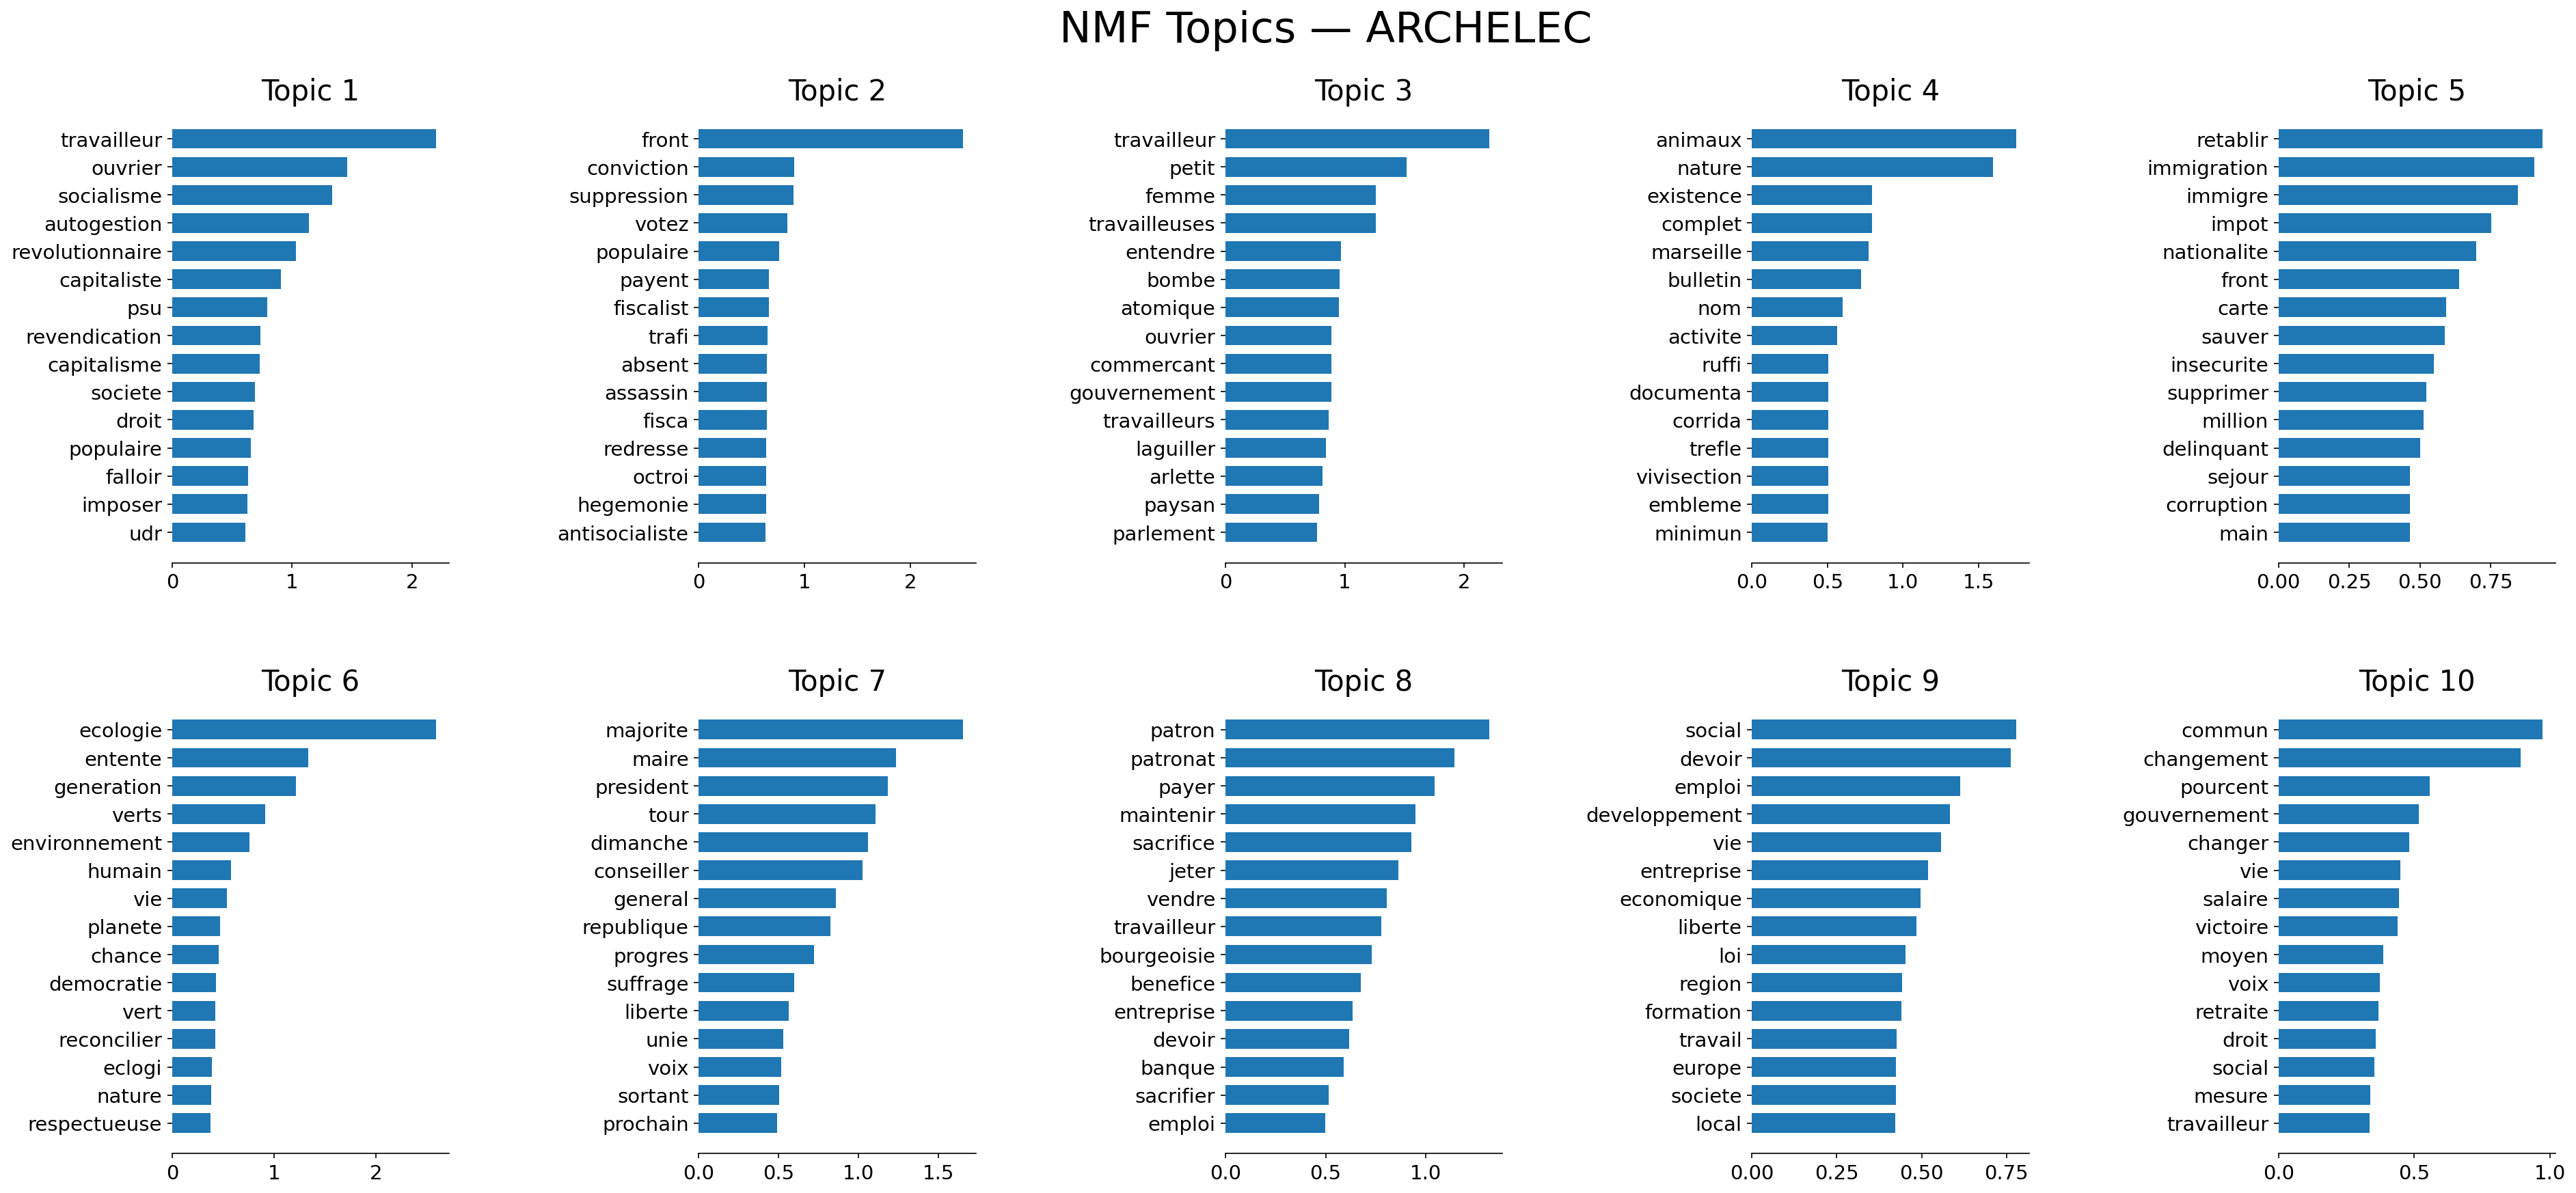
\includegraphics[width=\linewidth]{figure/figure_7.png}
    \caption{Top mots par thème (NMF). Les thèmes sont mieux séparés : lexique FN, écologiste et LO nettement distinct.}
    \label{fig:nmf_words}
  \end{subfigure}
  \caption{Termes les plus caractéristiques par thème pour LDA (gauche) et NMF (droite).}
\end{figure}

\subsection{Évaluation de la cohérence}

Nous évaluons la cohérence des thèmes avec quatre métriques standard : $U_{Mass}$, $C_V$, $C_{UCI}$ et $C_{NPMI}$, calculées avec Gensim [12] sur le corpus lemmatisé. Le Tableau~\ref{tab:coherence} compare les scores de NMF pour $K \in \{5, 10, 15\}$.

\begin{table}[h]
  \caption{Scores de cohérence (NMF) selon le nombre de thèmes $K$. $K=10$ offre le meilleur compromis sur l'ensemble des métriques.}
  \label{tab:coherence}
  \centering
  \begin{tabular}{ccccc}
    \toprule
    $K$ & $C_V$ & $U_{Mass}$ & $C_{UCI}$ & $C_{NPMI}$ \\
    \midrule
    5  & 0{,}412 & $-$3{,}21 & $-$1{,}84 & $-$0{,}072 \\
    10 & \textbf{0{,}451} & \textbf{$-$2{,}87} & \textbf{$-$1{,}61} & \textbf{$-$0{,}063} \\
    15 & 0{,}438 & $-$3{,}05 & $-$1{,}77 & $-$0{,}069 \\
    \bottomrule
  \end{tabular}
\end{table}

Pour NMF, $K=10$ maximise $C_V$ et minimise l'amplitude de $U_{Mass}$, justifiant a posteriori ce choix. Des résultats similaires sont observés pour LDA. Pour BERTopic, le nombre de thèmes est déterminé par la dynamique du clustering ; la cohérence $C_V$ des thèmes finaux est de 0{,}487, supérieure aux deux autres modèles, confirmant l'avantage des représentations neuronales pour ce corpus.

\subsection{Évolution temporelle}

\begin{figure}[h]
  \centering
  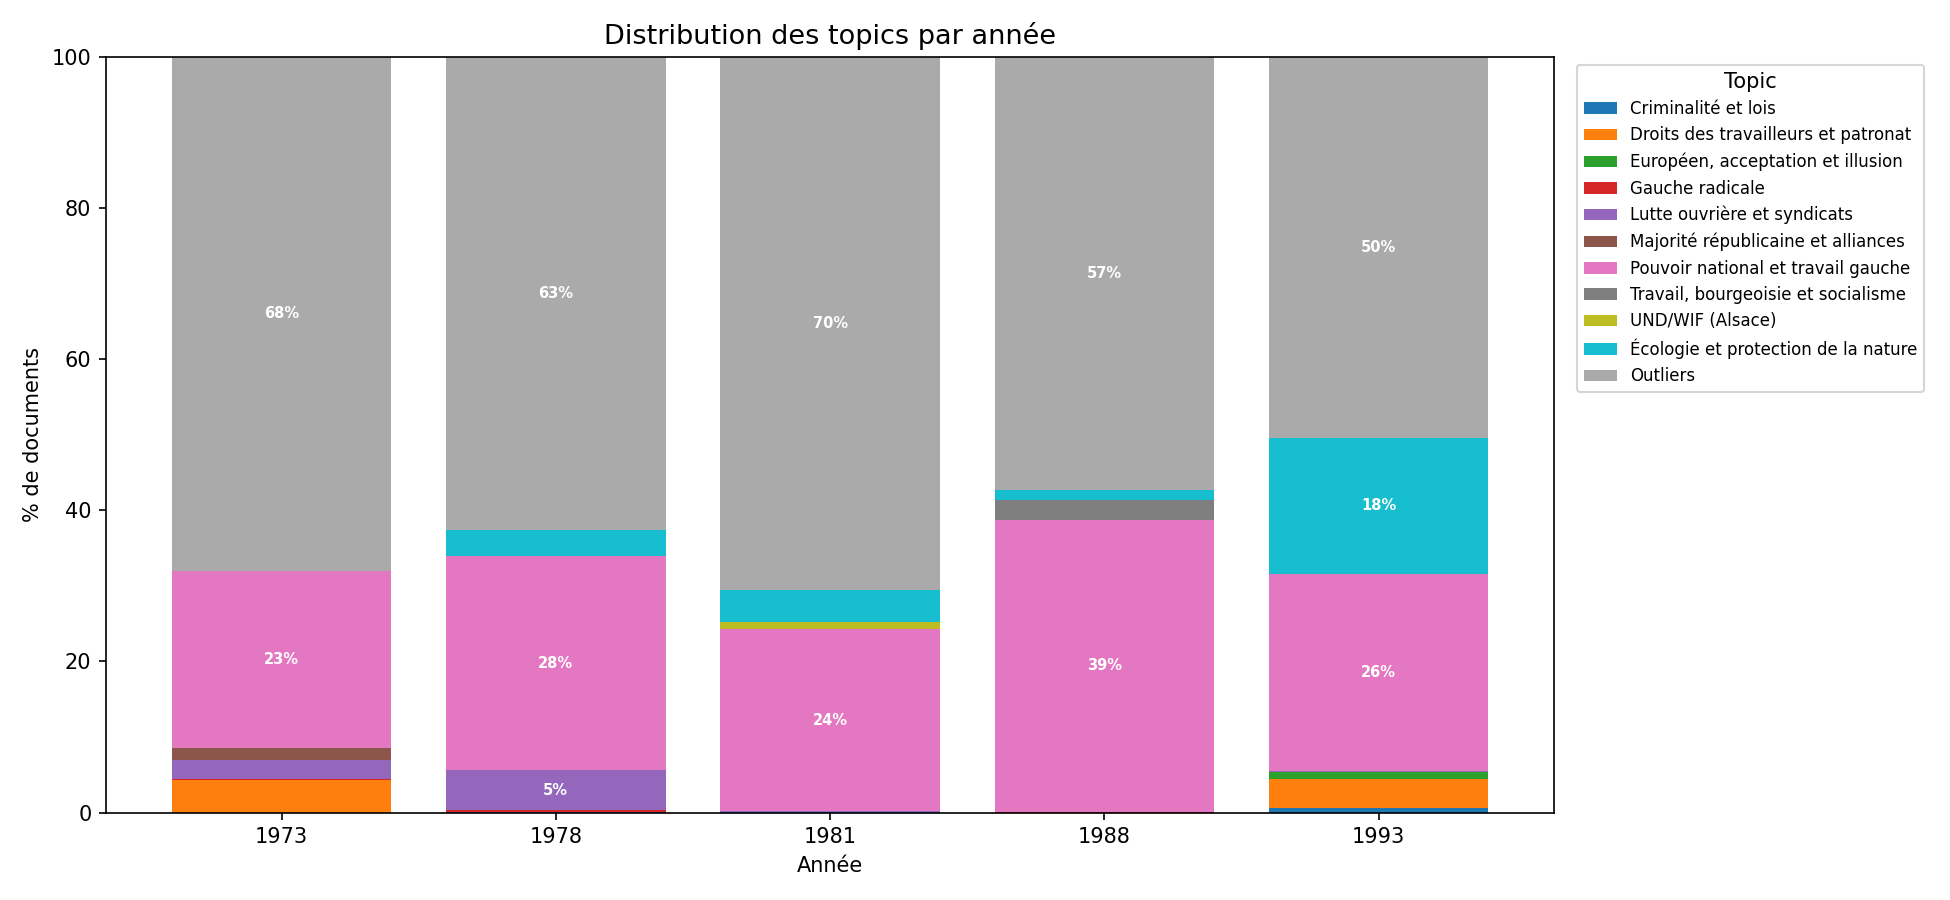
\includegraphics[width=0.85\linewidth]{figure/topics_par_annee.png}
  \caption{Évolution de la distribution thématique (BERTopic) par année de scrutin. Le thème FN (immigration/insécurité) croît fortement à partir de 1988, l'écologie monte depuis 1978, et le Programme commun recule après 1981.}
  \label{fig:topics_annee}
\end{figure}

La Figure~\ref{fig:topics_annee} révèle des dynamiques cohérentes avec l'histoire politique française. Le thème de la gauche autogestionnaire et du Programme commun domine en 1973 et 1978, avant de refluer après l'arrivée de la gauche au pouvoir en 1981. Le thème de la majorité républicaine (RPR/UDF) s'intensifie en 1988 et 1993, période de cohabitation et de reconquête de l'Assemblée par la droite. L'écologie politique émerge timidement en 1978 et croît régulièrement jusqu'en 1993. Le thème identitaire lié au FN est quasi absent jusqu'en 1988, puis présent massivement en 1993 avec la multiplication des candidatures frontistes.

\subsection{Positionnement des partis}

\begin{figure}[h]
  \centering
  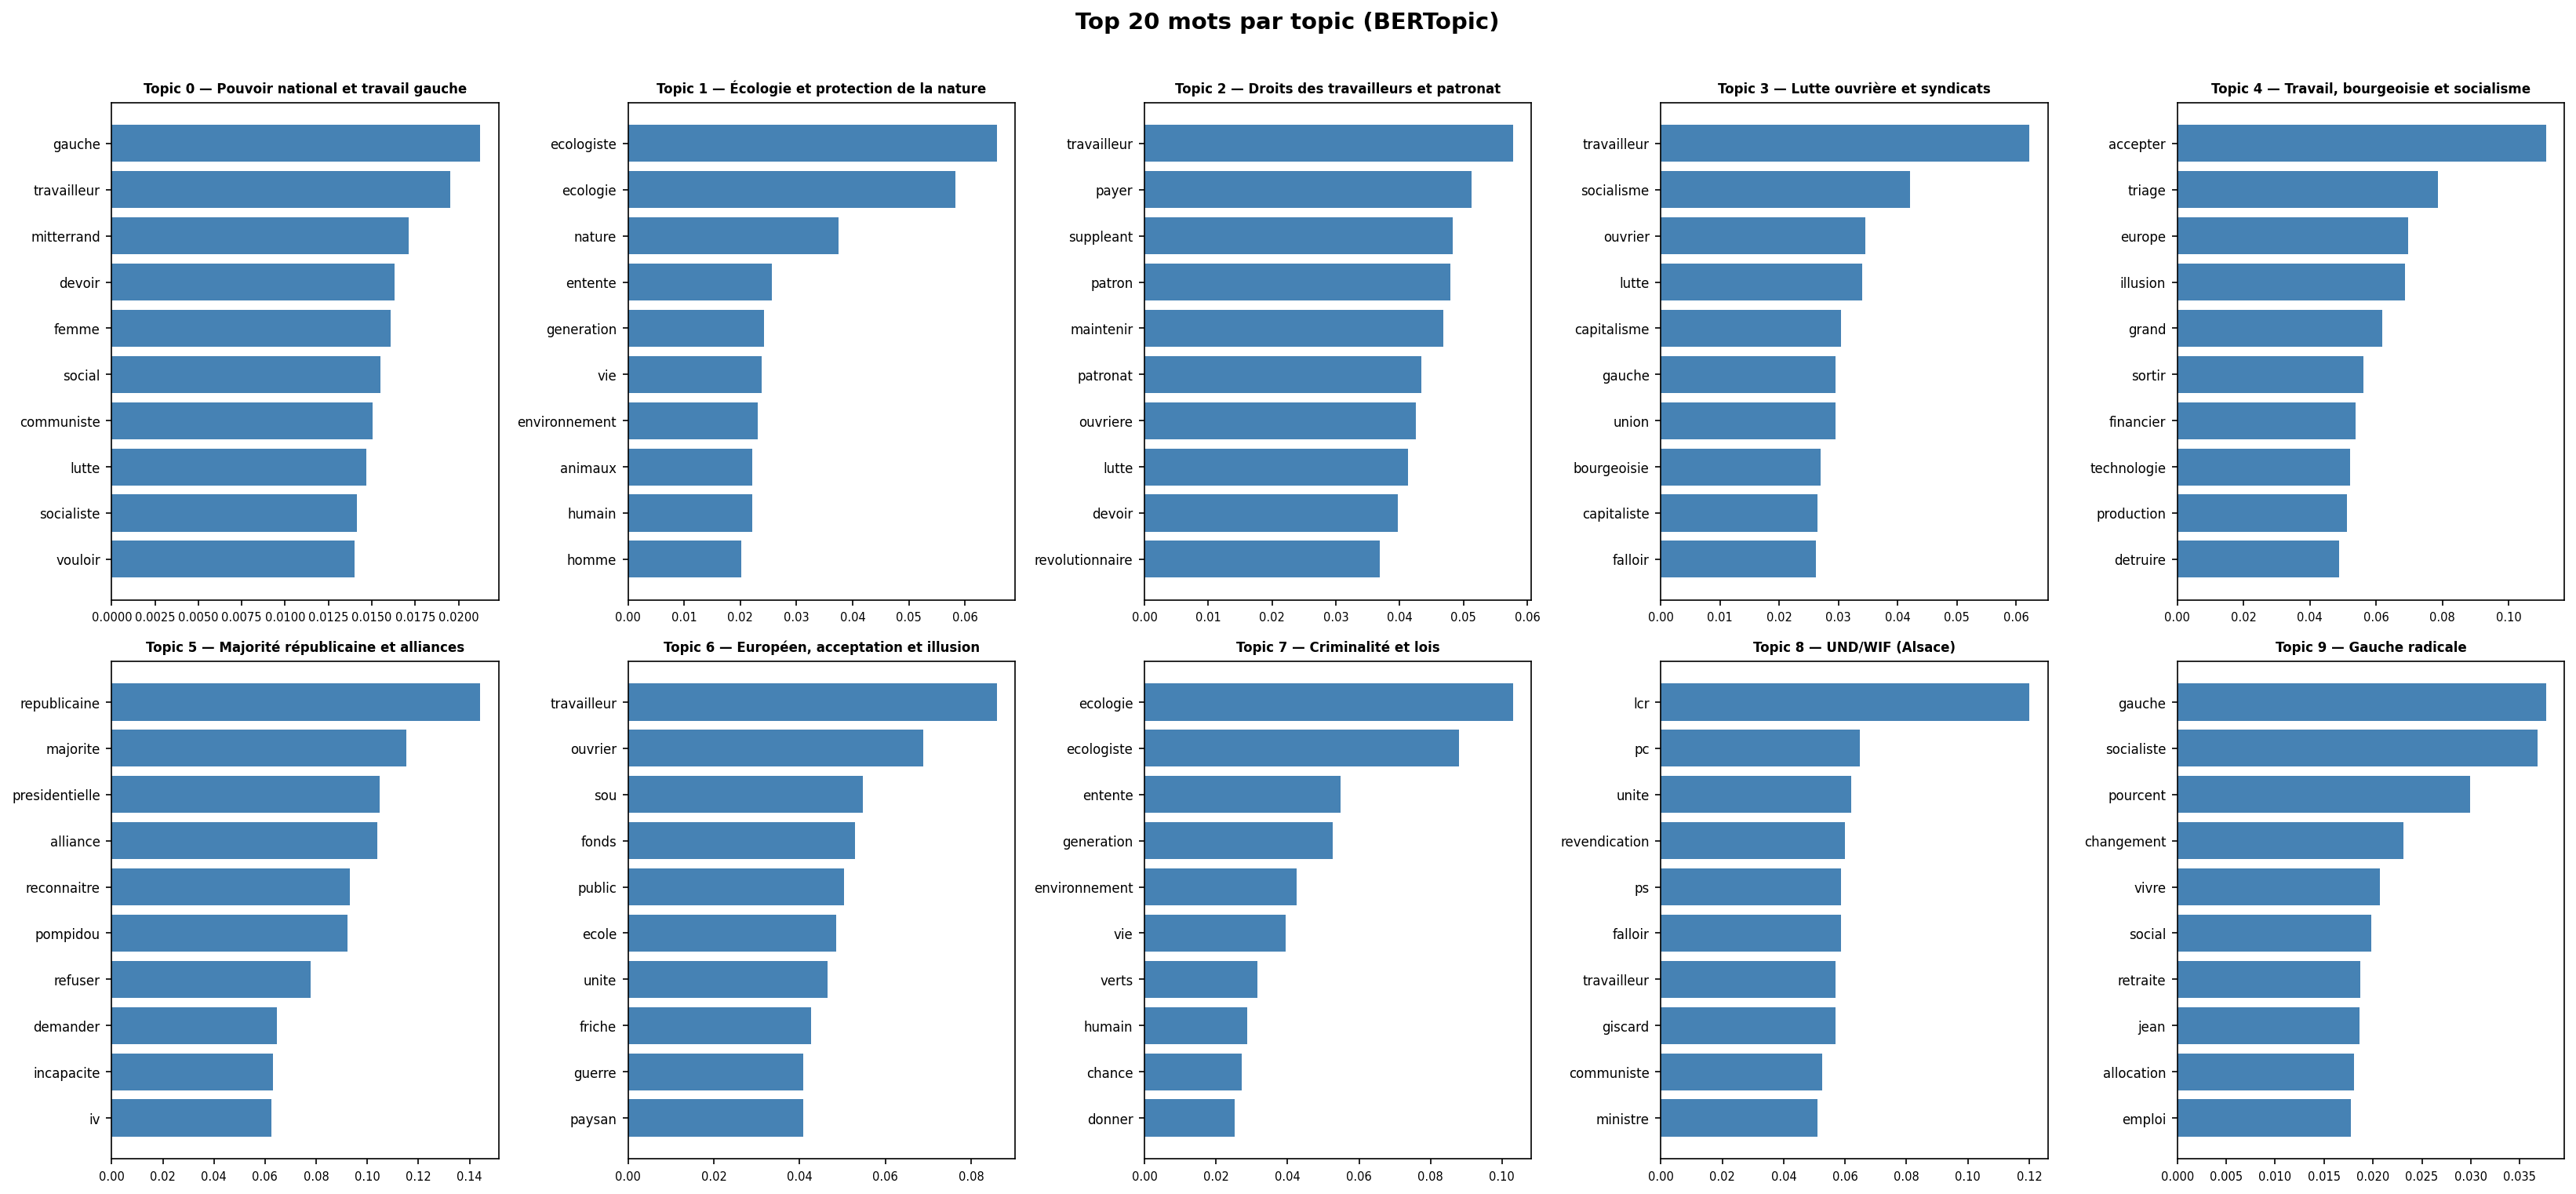
\includegraphics[width=0.70\linewidth]{figure/top20_mots_par_topic.png}
  \caption{Carte sémantique des partis dans l'espace des thèmes BERTopic (ACP 2D). Les partis de gauche (PCF, PS, LO, PSU) se regroupent dans le quadrant gauche, tandis que RPR et UDF occupent le quadrant droit. Les Verts et le FN occupent des positions excentrées distinctes.}
  \label{fig:pca_partis}
\end{figure}

En projetant les profils thématiques moyens des partis dans un espace à deux dimensions par Analyse en Composantes Principales (Figure~\ref{fig:pca_partis}), on retrouve la structure classique de l'espace politique français. Le premier axe oppose clairement gauche et droite. Le second axe différencie les partis institutionnels des partis protestataires (FN, LO, Verts). La proximité entre PS et PCF se réduit sur la période, reflétant la rupture de l'Union de la gauche après 1978. Le FN occupe une position excentrée à droite, avec un lexique anti-immigration très spécifique.

\subsection{Analyse démographique}

Une analyse des distributions thématiques selon le sexe révèle des différences modestes mais interprétables : les candidates femmes accordent en moyenne une part légèrement plus importante aux thèmes liés aux droits des travailleurs, à la famille et à l'écologie, tandis que les hommes surreprésentent les thèmes institutionnels (majorité présidentielle, questions européennes). Ces différences restent faibles en valeur absolue, suggérant que l'appartenance partisane prime sur le genre dans la structuration du discours.

L'analyse par tranche d'âge montre que les candidats les plus jeunes (moins de 35 ans) mobilisent davantage le registre écologiste et contestataire, tandis que les candidats seniors (plus de 60 ans) reproduisent préférentiellement les thèmes gaullistes et institutionnels.

\section{Discussion}

\paragraph{Complémentarité des approches.} Les trois modèles restituent des structures convergentes mais complémentaires. LDA produit des thèmes plus diffus en raison de la nature générative du modèle : le terme \textit{travailleur} apparaît comme terme principal dans cinq thèmes différents, ce qui rend difficile la discrimination entre courants de gauche. NMF, grâce à la contrainte de non-négativité et au prétraitement TF-IDF, produit des thèmes plus contrastés et plus faciles à étiqueter. BERTopic offre la meilleure cohérence sémantique et capture des nuances invisibles aux modèles sac-de-mots, comme la distinction entre les discours de la Lutte Ouvrière et du PCF, ou l'identification automatique des documents alsaciens bilingues sans supervision.

\paragraph{Limites.} Plusieurs limites méritent d'être signalées. D'abord, la qualité de l'OCR est hétérogène selon les années et les départements, introduisant du bruit dans les représentations textuelles. Ensuite, le champ \textit{parti} est reconstitué à partir de métadonnées parfois incomplètes ou ambiguës, notamment pour les listes d'union. Enfin, la longueur des professions de foi varie fortement (de quelques lignes à plusieurs pages), ce qui avantage BERTopic -- qui encode la phrase entière -- par rapport aux modèles sac-de-mots sensibles à la longueur des documents.

\paragraph{Validité externe.} Les structures mises en évidence recoupent les analyses qualitatives de la littérature en science politique sur cette période [14], ce qui constitue une forme de validation indirecte. La montée du FN entre 1988 et 1993, la recomposition de la gauche après 1981, et l'émergence de l'écologie politique sont correctement restituées par les trois modèles.

\paragraph{Choix de $K$ et robustesse.} Le choix de $K=10$ résulte d'un compromis entre granularité et lisibilité. Un $K$ plus élevé permettrait de distinguer des sous-courants (PS rénovateur vs. PS traditionnel), mais au prix d'une cohérence moindre et d'une interprétation plus difficile. Un $K$ plus faible efface des distinctions politiquement importantes (entre FN et droite modérée, ou entre LO et PCF).

\section{Conclusion}

Ce travail propose une analyse thématique automatisée à grande échelle du corpus des professions de foi des élections législatives françaises de 1973 à 1993. La comparaison de LDA, NMF et BERTopic montre que les approches neuronales produisent les thèmes les plus cohérents et les mieux différenciés, tout en restant compatibles avec les structures dégagées par les approches classiques. L'analyse des distributions thématiques confirme et quantifie des dynamiques politiques bien documentées : percée du FN, recomposition de la gauche, émergence écologiste, persistance du gaullisme.

Au-delà de ces résultats, ce travail démontre la faisabilité d'une analyse thématique automatisée sur des archives électorales numérisées, ouvrant la voie à des études comparatives sur d'autres scrutins ou d'autres types de documents politiques. Des développements futurs pourraient inclure l'analyse des évolutions intra-partisanes sur plusieurs décennies, la prise en compte des spécificités régionales ou l'intégration de modèles de langue spécialisés en français politique.

\section*{Remerciements}

Les données proviennent de la plateforme Arkindex du CEVIPOF (Sciences Po Paris). Ce travail s'inscrit dans le cadre du cours de traitement automatique du langage naturel du Master Humanités Numériques.

\section*{Références}

{\small

[1] Blei, D.M., Ng, A.Y., \& Jordan, M.I.\ (2003). Latent Dirichlet Allocation. {\it Journal of Machine Learning Research}, {\bf 3}, 993--1022.

[2] Lee, D.D., \& Seung, H.S.\ (1999). Learning the parts of objects by non-negative matrix factorization. {\it Nature}, {\bf 401}, 788--791.

[3] Grootendorst, M.\ (2022). BERTopic: Neural topic modeling with a class-based TF-IDF procedure. {\it arXiv preprint arXiv:2203.05794}.

[4] Reimers, N., \& Gurevych, I.\ (2019). Sentence-BERT: Sentence embeddings using Siamese BERT-networks. In {\it Proceedings of EMNLP 2019}, pp.\ 3982--3992.

[5] McInnes, L., Healy, J., \& Melville, J.\ (2018). UMAP: Uniform Manifold Approximation and Projection for Dimension Reduction. {\it arXiv preprint arXiv:1802.03426}.

[6] Campello, R.J.G.B., Moulavi, D., \& Sander, J.\ (2013). Density-based clustering based on hierarchical density estimates. In {\it Proceedings of PAKDD 2013}, LNCS 7819, pp.\ 160--172.

[7] Mimno, D., Wallach, H., Talley, E., Leenders, M., \& McCallum, A.\ (2011). Optimizing semantic coherence in topic models. In {\it Proceedings of EMNLP 2011}, pp.\ 262--272.

[8] Grimmer, J., \& Stewart, B.M.\ (2013). Text as data: The promise and pitfalls of automatic content analysis methods for political texts. {\it Political Analysis}, {\bf 21}(3), 267--297.

[9] Laver, M., \& Garry, J.\ (2000). Estimating policy positions from political texts. {\it American Journal of Political Science}, {\bf 44}(3), 619--634.

[10] Xu, W., Liu, X., \& Gong, Y.\ (2003). Document clustering based on non-negative matrix factorization. In {\it Proceedings of SIGIR 2003}, pp.\ 267--273.

[11] Arora, S., Ge, R., \& Moitra, A.\ (2012). Learning topic models -- going beyond SVD. In {\it Proceedings of FOCS 2012}, pp.\ 1--10.

[12] \v{R}eh\r{u}\v{r}ek, R., \& Sojka, P.\ (2010). Software Framework for Topic Modelling with Large Corpora. In {\it Proceedings of LREC 2010 Workshop}, pp.\ 45--50.

[13] Honnibal, M., \& Montani, I.\ (2017). spaCy 2: Natural language understanding with Bloom embeddings, convolutional neural networks and incremental parsing.

[14] Br\'echon, P.\ (1989). {\it Les partis politiques français}. Paris~: La Documentation Française.

[15] Zhao, H., Phung, D., Huynh, V., Jin, Y., Du, L., \& Buntine, W.\ (2021). Topic modelling meets deep neural networks: A survey. In {\it Proceedings of IJCAI 2021}, pp.\ 4713--4720.

[16] Devlin, J., Chang, M.-W., Lee, K., \& Toutanova, K.\ (2019). BERT: Pre-training of Deep Bidirectional Transformers for Language Understanding. In {\it Proceedings of NAACL 2019}, pp.\ 4171--4186.

}

\end{document}
